\documentclass[12pt]{article}
\usepackage{sbc-template}
\usepackage{graphicx,url}
\usepackage[brazil]{babel}   
%\usepackage[latin1]{inputenc}  
% Please add the following required packages to your document preamble:
% \usepackage{graphicx}
% Please add the following required packages to your document preamble:
% \usepackage{graphicx}

\usepackage{xcolor}
% Definindo novas cores
\definecolor{verde}{rgb}{0,0.5,0}
% Configurando layout para mostrar codigos C++
\usepackage{listings}
\lstset{
  language=C++,
  basicstyle=\ttfamily\small,
  keywordstyle=\color{blue},
  stringstyle=\color{verde},
  commentstyle=\color{red},
  extendedchars=true,
  showspaces=false,
  showstringspaces=false,
  numbers=left,
  numberstyle=\tiny,
  breaklines=true,
  backgroundcolor=\color{green!10},
  breakautoindent=true,
  captionpos=b,
  xleftmargin=0pt,
}
\pagestyle{empty}




\sloppy

\title{\textbf{Relatório}: Clusters}

\author{
    Romário Da S. Ferreira\inst{1},
    Luiz David Santin\inst{2},
    Lucas Nakamura\inst{3},
    Rafael Vellozo \inst{4}
}

\address{ Departamento Computação \\
        Universidade Tecnologica Federal do Paraná (UTFPR) 
        -- Medianeira, PR -- Brazil
        \email{{romario,lucasnakamura.1996}@alunos.utfpr.edu.br},
        \email{{luiz-santin@hotmail.com}},
        \email{rafaelldassilveira@gmail.com}
}

\begin{document} 

\maketitle

\section{Indrodução}
\subsection{Objetivos}

Criar e configurar um cluster para realização de trabalho de alto custo computacional para computadores convencionais, realizar testes de ordenação em arquivos de diversas tamanhos, fazendo assim observações sobre os resultados obtidos, onde tem-se como intenção ordenar arquivos com tamanho de linha diversos usando um algoritmo Bubble Sort paralelizado no qual foi disponibilizado na universidade de \textit{Heriot-Watt University} na Scotland, os arquivos contendo os valores a serem ordenados foram gerado por um script na linguagem c, no qual foi possível escolher o tamanho em linha do arquivo, possuindo como saída três arquivos, sendo eles randômico, ordenado e invertido.

\begin{itemize}
    \item Criar e configurar um cluster;
    \item Executar um algoritmo paralelizável;
    \item Medir tempo de execução das tarefas;
    \item Apresentar as informações coletadas.
\end{itemize}

\section{Metodologia} \label{sec:firstpage}
\subsection{Materiais}

Foram utilizado neste experimento 3 computadores pertencentes a Universidade Tecnológica Federal do Paraná, onde os mesmos
possuem a mesma característica de hardware como descrito na Tabela \ref{tab:computersLabor}, usamos também um switch e três pendrives, bem como o sistema operativo Pelican HPC GNU Linux para criação do cluster.

\begin{table}[]
\centering
\label{tab:computersLabor}
\resizebox{\textwidth}{!}{%
\begin{tabular}{l|llll}
Máquina & Processador & Versão do BIOS & Memória física total: & Placa de Rede \\ \hline
Computador 1 & Intel64 Family 6 Model 42 Stepping 7 GenuineIntel $\sim$3100 Mhz & Dell Inc. A07, 10/09/2011 & 8.073 MB & \begin{tabular}[c]{@{}l@{}}2 NIC(s) instalado(s). \\ {[}01{]}: Intel(R) 82579LM Gigabit Network Connection \\ {[}02{]}: Realtek PCI GBE Family Controller\end{tabular} \\
Computador 2 & Intel64 Family 6 Model 42 Stepping 7 GenuineIntel $\sim$3100 Mhz & Dell Inc. A07, 10/09/2011 & 8.073 MB & \begin{tabular}[c]{@{}l@{}}2 NIC(s) instalado(s). \\ {[}01{]}: Intel(R) 82579LM Gigabit Network Connection \\ {[}02{]}: Realtek PCI GBE Family Controller\end{tabular} \\
Computador 3 & Intel64 Family 6 Model 42 Stepping 7 GenuineIntel $\sim$3100 Mhz & Dell Inc. A07, 10/09/2011 & 8.073 MB & \begin{tabular}[c]{@{}l@{}}2 NIC(s) instalado(s). \\ {[}01{]}: Intel(R) 82579LM Gigabit Network Connection \\ {[}02{]}: Realtek PCI GBE Family Controller\end{tabular}
\end{tabular}%
}
\caption{Configuração das máquinas utilizadas no cluster}
\end{table}


\subsection{Metódos}
    Para realização do cluster foi utilizado um sistema operacional próprio para tal tarefa, 
    assim sendo usamos os sistema operacional Pelican HPC GNU Linux, onde realizamos a instalação
    em um pendrive e o tornamos bootavél, partimos do principio da necessidade de existir um computador
    mestre e outros escravos, então assim o fizemos, iniciamos o computador mestre e o configuramos para que
    permitisse que os computadores escravos conectassem ao mestre, no início possuímos problemas com a conexão dos 
    nós escravos com o mestre, mas este problema foi corrigido realizando a configuração correta, então foi necessário 
    que realizássemos a configuração na BIOS de cadas computador escravo para que realizasse o boot via rede, está etapa fez com que 
    os problemas ocorridos com criptografia e permissões fossem evitados. Utilizamos o switch pois ele não é um servidor DHCP, caso
    fosse um servidor DHCP poderia ocasionar problemas no cluster, visto que o nó master é responsável por realizar a distribuição e gerenciamento dos ips.
   
    Foi configurada a inicialização dos três computadores utilizados neste experimento, onde o dois computadores
    escravos foram configurados para inicializar pela placa de rede NIC, enquanto o computador mestre foi configurado
    para inicializar pelo pendrive. Desta forma, quando o computador mestre inicializou pelo pendrive e carregou o sistema
    operacional, foi necessário realizar uma pequena configuração indicando em qual rede o cluster seria montado, permitindo
    que os computadores escravos carregassem o sistema operacional pela rede e evitando a necessidade de criar novos pendrives
    bootavéis para carregar o sistema \cite{pel1:995}.

    Necessitou-se realizar a compilação do algoritmo de ordenação e algoritmo de geração de arquivos a serem ordenados. Para isso, utilizou-se o compilador mpicc, o qual é especifico para compilar códigos paralelizados desenvolvidos em c. Também foi necessário fornecer parâmetros de entrada para que a compilação obtivesse sucesso, utilizar o compilador padrão gcc para realizar a compilação do programa que gera arquivos. Como exemplo, temos o comando \textbf{gcc program.c -o programResult} \cite{pel2:996}.

    Após realizado todo esse processo, realizou-se a execução de ambos programas. Primeiro gerou-se os arquivos necessários com tamanhos de 500000 e 100000 de linhas, depois foi executado o comando \textbf{mpirun -np num-processos program file-in file-out}, onde váriamos o número de processo de 16 até 256, após a variação de processos realizamos o desligamento 1 máquinas assim ficando com 2 máquinas ligadas e realizamos novamente o teste nos arquivos com 500000 linhas, após a conclusão da tarefa desligamos outra máquina assim ficando com somente uma ativa no cluster e voltamos a realizar o teste \cite{pel13:997}.
    
    % Please add the following required packages to your document preamble:
% \usepackage{graphicx}
\begin{table}[]
\centering

\label{tab:hpctest}
\resizebox{0.5\textwidth}{!}{%
    \begin{tabular}{ll}
        \multicolumn{2}{l}{HPC Test} \\ \hline
        \multicolumn{1}{l|}{Description} & Value \\ \hline
        \multicolumn{1}{l|}{Quantity of processors} & 6 \\
        \multicolumn{1}{l|}{Calculation time} & 0.48 seconds \\
        \multicolumn{1}{l|}{Cluster speed} & 3749 MFLOPS \\
        \multicolumn{1}{l|}{Cluster node N00 speed} & 624 MFLOPS \\
        \multicolumn{1}{l|}{Cluster node NO1 speed} & 628 MFLOPS \\
        \multicolumn{1}{l|}{Cluster node NO2 speed} & 1180 MFLOPS \\
        \multicolumn{1}{l|}{Cluster node NO3 speed} & 995 MFLOPS \\
        \multicolumn{1}{l|}{Cluster node N04 speed} & 624 MFLOPS \\
        \multicolumn{1}{l|}{Cluster node NO5 speed} & 878 MFLOPS
    \end{tabular}%
}
\caption{Apresenta a quantidade de processadores disponíveis no cluster, bem como a capacidade de cada nó em realizar os cálculos.}
\end{table}
    
    
    \begin{figure}[!htb]
         \centering
         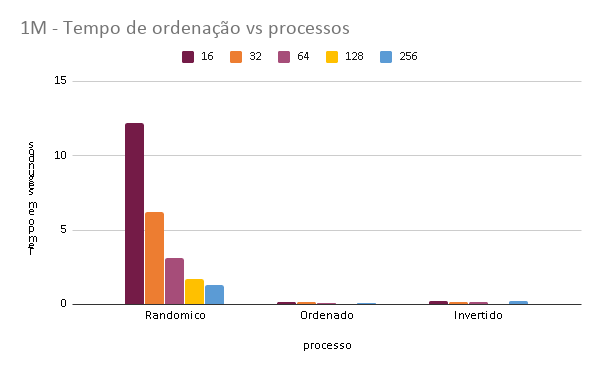
\includegraphics[scale=.5]{chart/chart1.png}
         \caption{Apresenta os tipos de arquivos ordenados de acordo com cada processo vs o tempo consumido para realizar a tarefa, onde os arquivos possuem o tamanho de 1 Milhão de linhas.}
         \label{img:chart1}
    \end{figure}
   
    \begin{figure}[!htb]
         \centering
         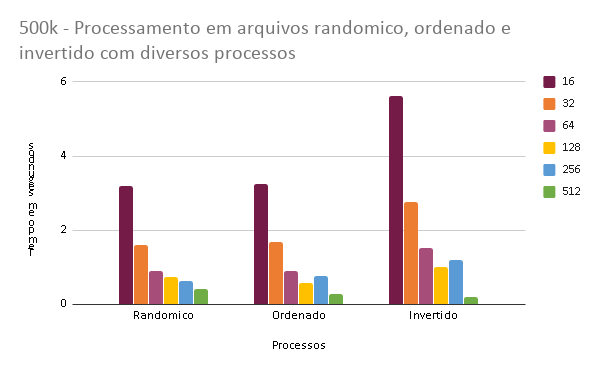
\includegraphics[scale=.5]{chart/chart2.png}
         \caption{Apresenta os tipos de arquivos ordenados de acordo com cada processo vs o tempo consumido para realizar a tarefa, onde os arquivos possuem 500 mil linhas.}
         \label{img:chart2}
    \end{figure}
   
    \begin{figure}[!htb]
         \centering
         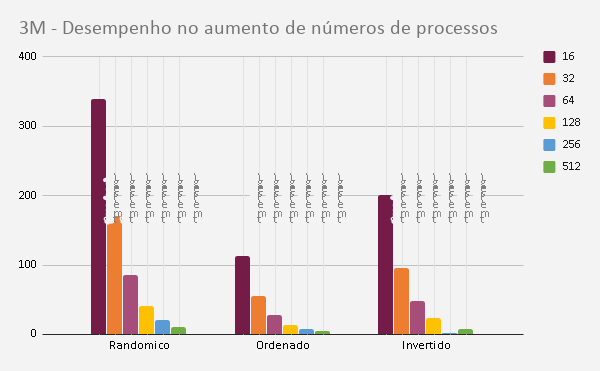
\includegraphics[scale=0.5]{chart/chart3.png}
         \caption{Apresenta os tipos de arquivos ordenados de acordo com cada processo vs o tempo consumido para realizar a tarefa, onde os arquivos possuem 3 Milhões linhas.}
         \label{img:chart3}
    \end{figure}
   
    \begin{figure}[!htb]
         \centering
         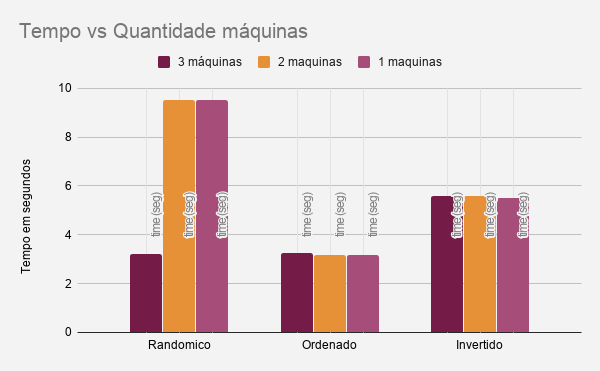
\includegraphics[scale=0.5]{chart/chart4.png}
         \caption{Apresenta os tipos de arquivos ordenados de acordo com um número limitado a 16 processos
         vs o tempo consumido para realizar a tarefa, onde os arquivos possuem 500 mil linhas, neste caso os nós escravos foram desligados no decorrer do teste.}
         \label{img:chart4}
    \end{figure}
   
    
    


\section{Resultados e discussões}

Quando foram utilizadas três máquinas para a ordenar os valores, o arquivo aleatório foi o que mais se destacou pelo fato de que, quando o número de processos era menor, mais rápido foi ordenado, mas quando atingia o número de 512 processos, o desempenho diminuiu. Contudo, utilizando duas máquinas escravas e uma máquina mestra, no total de 16 processos, os valores ficaram maiores apesar de que utilizando apenar uma maquina o desempenho ficou melhor que utilizar duas máquinas, exceto quando tentou ordenar o arquivo randômico, obtendo uma grande redução de desempenho, por requisitar mais do processador. Ao utilizar um algoritmo não paralelizável, o master fazia a utilização de 1 núcleo por vez e assim consumindo muito tempo entre as operações requisitadas.

Foi possível observar na comparação com quantidade de máquinas que é apresentado na Figura \ref{img:chart4}, que para o 
caso com 3 máquinas os valores tem pouca diferença entre o randômico e ordenado, porém os valores invertido houve um tempo maior de processamento, levando em consideração os arquivos com tamanho de 500 mil linhas. Para o caso de duas máquinas é possível notar grande discrepância se comparado a três máquinas, visto que em três maquinas o tempo de processamento do arquivo randômico foi de 3,197146/s, já no caso de duas máquinas o tempo de processamento foi de 9,499939/s, assim ficando com uma diferença de 6.302793/s, para ambos casos foram utilizados 16 processos paralelos.

Foi possível notar que não houve diferença significativas entre o caso de uma máquina e duas máquinas, pois a diferença no tempo de processamento foi muito pequena levando em consideração que neste casos foram utilizados 16 processos com arquivos com 500 mil linhas.

Notamos que se tivéssemos utilizado as placas de redes off-board instaladas nas máquinas poderíamos ter um desempenho melhor, visto que a placa on-board que utilizamos era limitada a 100Mb/s, se levarmos em consideração a rede, ao utilizarmos as placas 1Gb/s teriamos uma taxa de transfêrencia maior, onde por sua vez poderia evitar um possível gargalo na transmissão dos dados.



\begin{table}[]
\begin{tabular}{l|llllll}
           &                 &                     & Tipo de Arquivos  &            &            \\  \hline
           &                 &                     & Tempo em segundos &            &            \\ \hline
        & Linhas     & N. Processos      & Randômico         & Ordenado   & Invertido  \\ \hline
3 maquinas & 3000000    & 16              & 339,132014          & 113,058303        & 200,285386 \\
3 maquinas & 3000000    & 32              & 170,791132          & 55,598693         & 95,987929  &            \\
3 maquinas & 3000000    & 64              & 85,345131           & 27,42872          & 47,990014  &            \\
3 maquinas & 3000000    & 128             & 40,430747           & 13,701426         & 24,039388  &            \\
3 maquinas & 3000000    & 256             & 20,167077           & 7,328713          & 2,608632   &            \\
3 maquinas & 3000000    & 512             & 11,055823           & 5,206665          & 7,890164   &            \\
3 maquinas & 1000000    & 16              & 12,185057           & 0,154966          & 0,254218   &            \\
3 maquinas & 1000000    & 32              & 6,213659            & 0,138077          & 0,162084   &            \\
3 maquinas & 1000000    & 64              & 3,139923            & 0,080498          & 0,154480   &            \\
3 maquinas & 1000000    & 128             & 1,738475            & 0,028435          & 0,037343   &            \\
3 maquinas & 1000000    & 256             & 1,338091            & 0,078705          & 0,208795   &            \\
3 maquinas & 1000000    & 512             & 1,816653            & Erro              & Erro       &            \\
3 maquinas & 500000     & 16              & 3,197146            & 3,240204          & 5,608355   &            \\
3 maquinas & 500000     & 32              & 1,609271            & 1,672758          & 2,753006   &            \\
3 maquinas & 500000     & 64              & 0,892058            & 0,898319          & 1,516231   &            \\
3 maquinas & 500000     & 128             & 0,731357            & 0,566566          & 1,021335   &            \\
3 maquinas & 500000     & 256             & 0,639991            & 0,771383          & 1,204545   &            \\
3 maquinas & 500000     & 512             & 0,408242            & 0,277766          & 0,213484   &            \\
2 maquinas & 500000          & 16                  & 9,499939          & 3,158108   & 5,570042   \\
1 maquinas & 500000          & 16                  & 9,531287          & 3,157503   & 5,493562  
\end{tabular}
\caption{Tabela dos resultados obtidos ao processar os arquivos no cluster}
\label{tab:table-result-cluster}
\end{table}
\section{Conclusões}

Concluiu-se que a utilização do Pelican HPC como forma de criar e configurar as máquinas em cluster, tornou o projeto facilmente viável e de fácil configuração e manutenção, embora tenham ocorridos dificuldades na configuração inicial do nós escravos para o mestre, após obtido o devido conhecimento sobre o sistema em especifico a configuração dos nós escravos via rede.

É importante ressaltar que em nosso caso especifico notou-se que a utilização de cluster só se faz necessário se houver grandes 
quantidades de dados para processamento, visto que em função da diminuição da quantidade de dados a serem processados o cluster 
acaba perdendo seu poder computacional, compreendeu-se que a rede pode ser um empecilho em determinados casos, onde existam firewall filtrando os pacotes das redes.

Em relação aos dados observou-se que quanto mais paralelizável for suas tarefas mais rápido ela será solucionada, como mostrado nos gráficos da Figura \ref{img:chart2} e \ref{img:chart3}, podemos afirmar que existe uma relação na qual diz que na medida em que aumenta os processos o tempo de execução das tarefas diminuem.

Após todos os testes realizados conclui-se que a utilização do cluster realmente traz um beneficio computacional, visto permite-se obter um valor computacional alto com custo financeiro baixo, assim permitindo a pessoas com pouco poder aquisitivo realizar experimentos científicos no ramos da ciência que exijam grandes quantidades de processamentos.

\bibliographystyle{sbc}

\bibliography{sbc-template}


\newpage
 Código do Bubble Sort paralelizado obtido da Heriot-Watt University Edinburgh, Scotland, UK EH14 4AS, pelo link \url{http://www.macs.hw.ac.uk/~hwloidl/Courses/F21DP/srcs/bsort.c}
\begin{lstlisting}
/* 
   bsort.c - Parallel sorting algorithm based on bubblesort

   compile: mpicc -Wall -O -o bsort bsort.c
   run:     mpirun -np num_procs bsort in_file out_file
*/

#include <stdio.h>
#include <stdlib.h>
#include <mpi.h>


/* swap entries in array v at positions i and j; used by bubblesort */
static inline /* this improves performance; Exercise: by how much? */
void swap(int * v, int i, int j)
{
  int t = v[i];
  v[i] = v[j];
  v[j] = t;
}


/* (bubble) sort array v; array is of length n */
void bubblesort(int * v, int n)
{
  int i, j;
  for (i = n-2; i >= 0; i--)
    for (j = 0; j <= i; j++)
      if (v[j] > v[j+1])
        swap(v, j, j+1);
}


/* merge two sorted arrays v1, v2 of lengths n1, n2, respectively */
int * merge(int * v1, int n1, int * v2, int n2)
{
  int * result = (int *)malloc((n1 + n2) * sizeof(int));
  int i = 0;
  int j = 0;
  int k;
  for (k = 0; k < n1 + n2; k++) {
    if (i >= n1) {
      result[k] = v2[j];
      j++;
    }
    else if (j >= n2) {
      result[k] = v1[i];
      i++;
    }
    else if (v1[i] < v2[j]) { // indices in bounds as i < n1 && j < n2
      result[k] = v1[i];
      i++;
    }
    else { // v2[j] <= v1[i]
      result[k] = v2[j];
      j++;
    }
  }
  return result;
}


int main(int argc, char ** argv)
{
  int n;
  int * data = NULL;
  int c, s;
  int * chunk;
  int o;
  int * other;
  int step;
  int p, id;
  MPI_Status status;
  double elapsed_time;
  FILE * file = NULL;
  int i;

  if (argc!=3) {
    fprintf(stderr, "Usage: mpirun -np <num_procs> %s <in_file> <out_file>\n", argv[0]);
    exit(1);
  }

  MPI_Init(&argc, &argv);
  MPI_Comm_size(MPI_COMM_WORLD, &p);
  MPI_Comm_rank(MPI_COMM_WORLD, &id);

  if (id == 0) {
    // read size of data
    file = fopen(argv[1], "r");
    fscanf(file, "%d", &n);
    // compute chunk size
    c = n/p; if (n%p) c++;
    // read data from file
    data = (int *)malloc(p*c * sizeof(int));
    for (i = 0; i < n; i++)
      fscanf(file, "%d", &(data[i]));
    fclose(file);
    // pad data with 0 -- doesn't matter
    for (i = n; i < p*c; i++)
      data[i] = 0;
  }

  // start the timer
  MPI_Barrier(MPI_COMM_WORLD);
  elapsed_time = - MPI_Wtime();

  // broadcast size
  MPI_Bcast(&n, 1, MPI_INT, 0, MPI_COMM_WORLD);

  // compute chunk size
  c = n/p; if (n%p) c++;

  // scatter data
  chunk = (int *)malloc(c * sizeof(int));
  MPI_Scatter(data, c, MPI_INT, chunk, c, MPI_INT, 0, MPI_COMM_WORLD);
  free(data);
  data = NULL;

  // compute size of own chunk and sort it
  s = (n >= c * (id+1)) ? c : n - c * id;
  bubblesort(chunk, s);

  // up to log_2 p merge steps
  for (step = 1; step < p; step = 2*step) {
    if (id % (2*step)!=0) {
      // id is no multiple of 2*step: send chunk to id-step and exit loop
      MPI_Send(chunk, s, MPI_INT, id-step, 0, MPI_COMM_WORLD);
      break;
    }
    // id is multiple of 2*step: merge in chunk from id+step (if it exists)
    if (id+step < p) {
      // compute size of chunk to be received
      o = (n >= c * (id+2*step)) ? c * step : n - c * (id+step);
      // receive other chunk
      other = (int *)malloc(o * sizeof(int));
      MPI_Recv(other, o, MPI_INT, id+step, 0, MPI_COMM_WORLD, &status);
      // merge and free memory
      data = merge(chunk, s, other, o);
      free(chunk);
      free(other);
      chunk = data;
      s = s + o;
    }
  }

  // stop the timer
  elapsed_time += MPI_Wtime();

  // write sorted data to out file and print out timer
  if (id == 0) {
    file = fopen(argv[2], "w");
    fprintf(file, "%d\n", s);   // assert (s == n)
    for (i = 0; i < s; i++)
      fprintf(file, "%d\n", chunk[i]);
    fclose(file);
    printf("Bubblesort %d ints on %d procs: %f secs\n", n, p, elapsed_time);
    // printf("%d %2d %f\n", n, p, elapsed_time);
  }

  MPI_Finalize();
  return 0;
} \end{lstlisting}
\end{document}
